\begin{figure}[h]
	\centering
		 \resizebox{0.5\textwidth}{!}{
		
\tikzset{every picture/.style={line width=0.75pt}} %set default line width to 0.75pt

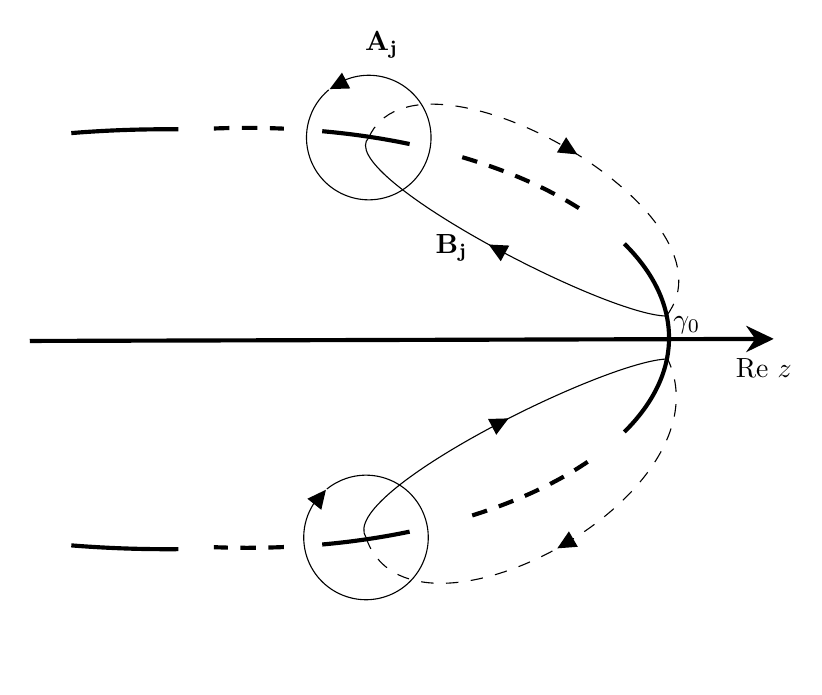
\begin{tikzpicture}[x=0.75pt,y=0.75pt,yscale=-1,xscale=1]
	%uncomment if require: \path (0,404); %set diagram left start at 0, and has height of 404
	
	%Straight Lines [id:da7223098994070081]
	\draw [fill={rgb, 255:red, 155; green, 155; blue, 155 }  ,fill opacity=1 ][line width=1.5]    (165,201) -- (519.45,200.01) ;
	\draw [shift={(523.45,200)}, rotate = 179.84] [fill={rgb, 255:red, 0; green, 0; blue, 0 }  ][line width=0.08]  [draw opacity=0] (13.4,-6.43) -- (0,0) -- (13.4,6.44) -- (8.9,0) -- cycle    ;
	%Shape: Arc [id:dp7197767916689966]
	\draw  [draw opacity=0][dash pattern={on 5.63pt off 4.5pt}][line width=1.5]  (287.44,300.29) .. controls (281.58,300.54) and (275.65,300.67) .. (269.67,300.67) .. controls (264.29,300.67) and (258.96,300.56) .. (253.69,300.36) -- (269.67,199.5) -- cycle ; \draw  [dash pattern={on 5.63pt off 4.5pt}][line width=1.5]  (287.44,300.29) .. controls (281.58,300.54) and (275.65,300.67) .. (269.67,300.67) .. controls (264.29,300.67) and (258.96,300.56) .. (253.69,300.36) ;
	%Shape: Arc [id:dp3653236378506848]
	\draw  [draw opacity=0][line width=1.5]  (451.49,154.17) .. controls (465.25,167.8) and (473,183.2) .. (473,199.5) .. controls (473,215.8) and (465.25,231.2) .. (451.49,244.83) -- (269.67,199.5) -- cycle ; \draw  [line width=1.5]  (451.49,154.17) .. controls (465.25,167.8) and (473,183.2) .. (473,199.5) .. controls (473,215.8) and (465.25,231.2) .. (451.49,244.83) ;
	%Shape: Arc [id:dp9141977916603252]
	\draw  [draw opacity=0][dash pattern={on 5.63pt off 4.5pt}][line width=1.5]  (253.69,98.64) .. controls (258.96,98.44) and (264.29,98.33) .. (269.67,98.33) .. controls (275.65,98.33) and (281.58,98.46) .. (287.44,98.71) -- (269.67,199.5) -- cycle ; \draw  [dash pattern={on 5.63pt off 4.5pt}][line width=1.5]  (253.69,98.64) .. controls (258.96,98.44) and (264.29,98.33) .. (269.67,98.33) .. controls (275.65,98.33) and (281.58,98.46) .. (287.44,98.71) ;
	%Shape: Arc [id:dp018363651430338468]
	\draw  [draw opacity=0][line width=1.5]  (305.91,99.94) .. controls (320.55,101.25) and (334.65,103.34) .. (348.02,106.12) -- (269.67,199.5) -- cycle ; \draw  [line width=1.5]  (305.91,99.94) .. controls (320.55,101.25) and (334.65,103.34) .. (348.02,106.12) ;
	%Shape: Arc [id:dp7598335590527734]
	\draw  [draw opacity=0][line width=1.5]  (348.02,292.88) .. controls (334.65,295.66) and (320.55,297.75) .. (305.91,299.06) -- (269.67,199.5) -- cycle ; \draw  [line width=1.5]  (348.02,292.88) .. controls (334.65,295.66) and (320.55,297.75) .. (305.91,299.06) ;
	%Shape: Arc [id:dp5875638612610647]
	\draw  [draw opacity=0][dash pattern={on 5.63pt off 4.5pt}][line width=1.5]  (373.39,112.47) .. controls (397.04,119.46) and (417.59,128.77) .. (433.79,139.77) -- (269.67,199.5) -- cycle ; \draw  [dash pattern={on 5.63pt off 4.5pt}][line width=1.5]  (373.39,112.47) .. controls (397.04,119.46) and (417.59,128.77) .. (433.79,139.77) ;
	%Shape: Arc [id:dp17650732443428496]
	\draw  [draw opacity=0][dash pattern={on 5.63pt off 4.5pt}][line width=1.5]  (433.79,259.23) .. controls (417.59,270.23) and (397.04,279.54) .. (373.39,286.53) -- (269.67,199.5) -- cycle ; \draw  [dash pattern={on 5.63pt off 4.5pt}][line width=1.5]  (433.79,259.23) .. controls (417.59,270.23) and (397.04,279.54) .. (373.39,286.53) ;
	%Curve Lines [id:da482825425220228]
	\draw    (328.33,103) .. controls (311,120.33) and (441,188.33) .. (471.67,189) ;
	\draw [shift={(386.13,154.55)}, rotate = 28.52] [fill={rgb, 255:red, 0; green, 0; blue, 0 }  ][line width=0.08]  [draw opacity=0] (8.93,-4.29) -- (0,0) -- (8.93,4.29) -- cycle    ;
	%Curve Lines [id:da15864062625404984]
	\draw    (327,295.67) .. controls (313,274.33) and (442.33,210.33) .. (472.33,209.67) ;
	\draw [shift={(395.71,238.3)}, rotate = 152.67] [fill={rgb, 255:red, 0; green, 0; blue, 0 }  ][line width=0.08]  [draw opacity=0] (8.93,-4.29) -- (0,0) -- (8.93,4.29) -- cycle    ;
	%Shape: Arc [id:dp5867404631491058]
	\draw  [draw opacity=0][line width=1.5]  (185.02,100.85) .. controls (200.01,99.63) and (215.49,99) .. (231.33,99) .. controls (233.1,99) and (234.87,99.01) .. (236.63,99.02) -- (231.33,200.17) -- cycle ; \draw  [line width=1.5]  (185.02,100.85) .. controls (200.01,99.63) and (215.49,99) .. (231.33,99) .. controls (233.1,99) and (234.87,99.01) .. (236.63,99.02) ;
	%Shape: Arc [id:dp19861604303444103]
	\draw  [draw opacity=0][line width=1.5]  (236.63,301.31) .. controls (234.87,301.33) and (233.1,301.33) .. (231.33,301.33) .. controls (215.49,301.33) and (200.01,300.7) .. (185.02,299.49) -- (231.33,200.17) -- cycle ; \draw  [line width=1.5]  (236.63,301.31) .. controls (234.87,301.33) and (233.1,301.33) .. (231.33,301.33) .. controls (215.49,301.33) and (200.01,300.7) .. (185.02,299.49) ;
	%Curve Lines [id:da2194430446529394]
	\draw  [dash pattern={on 4.5pt off 4.5pt}]  (328.33,103) .. controls (351.67,50.33) and (510.33,139.67) .. (471.67,189) ;
	\draw [shift={(428.85,111.13)}, rotate = 211.12] [fill={rgb, 255:red, 0; green, 0; blue, 0 }  ][line width=0.08]  [draw opacity=0] (8.93,-4.29) -- (0,0) -- (8.93,4.29) -- cycle    ;
	%Curve Lines [id:da34362702277658097]
	\draw  [dash pattern={on 4.5pt off 4.5pt}]  (327,295.67) .. controls (347.67,357.67) and (503.67,276.33) .. (472.33,209.67) ;
	\draw [shift={(419.17,300.92)}, rotate = 330.04] [fill={rgb, 255:red, 0; green, 0; blue, 0 }  ][line width=0.08]  [draw opacity=0] (8.93,-4.29) -- (0,0) -- (8.93,4.29) -- cycle    ;
	%Shape: Arc [id:dp11287113090264955]
	\draw  [draw opacity=0] (308.15,272.32) .. controls (310.8,270.18) and (313.86,268.46) .. (317.27,267.29) .. controls (332.95,261.92) and (350.01,270.27) .. (355.38,285.94) .. controls (360.75,301.61) and (352.4,318.67) .. (336.73,324.05) .. controls (321.05,329.42) and (303.99,321.07) .. (298.62,305.39) .. controls (294.49,293.33) and (298.48,280.45) .. (307.68,272.7) -- (327,295.67) -- cycle ; \draw    (308.15,272.32) .. controls (310.8,270.18) and (313.86,268.46) .. (317.27,267.29) .. controls (332.95,261.92) and (350.01,270.27) .. (355.38,285.94) .. controls (360.75,301.61) and (352.4,318.67) .. (336.73,324.05) .. controls (321.05,329.42) and (303.99,321.07) .. (298.62,305.39) .. controls (294.82,294.3) and (297.89,282.5) .. (305.58,274.66) ; \draw [shift={(307.68,272.7)}, rotate = 128.59] [fill={rgb, 255:red, 0; green, 0; blue, 0 }  ][line width=0.08]  [draw opacity=0] (8.93,-4.29) -- (0,0) -- (8.93,4.29) -- cycle    ;
	%Shape: Arc [id:dp9138993892223812]
	\draw  [draw opacity=0] (309.48,79.65) .. controls (312.13,77.51) and (315.2,75.79) .. (318.61,74.62) .. controls (334.28,69.25) and (351.34,77.6) .. (356.71,93.27) .. controls (362.08,108.95) and (353.73,126.01) .. (338.06,131.38) .. controls (322.39,136.75) and (305.33,128.4) .. (299.95,112.73) .. controls (295.82,100.67) and (299.81,87.78) .. (309.02,80.04) -- (328.33,103) -- cycle ; \draw    (311.93,77.87) .. controls (313.97,76.54) and (316.2,75.44) .. (318.61,74.62) .. controls (334.28,69.25) and (351.34,77.6) .. (356.71,93.27) .. controls (362.08,108.95) and (353.73,126.01) .. (338.06,131.38) .. controls (322.39,136.75) and (305.33,128.4) .. (299.95,112.73) .. controls (295.82,100.67) and (299.81,87.78) .. (309.02,80.04) ;  \draw [shift={(309.48,79.65)}, rotate = 332.61] [fill={rgb, 255:red, 0; green, 0; blue, 0 }  ][line width=0.08]  [draw opacity=0] (8.93,-4.29) -- (0,0) -- (8.93,4.29) -- cycle    ;
	
	% Text Node
	\draw (503.89,208) node [anchor=north west][inner sep=0.75pt]   [align=left] {$\mathrm{Re}\,\, z$};
	
	\draw (473.89,188) node [anchor=north west][inner sep=0.75pt]   [align=left] {$\gamma_0$};
	% Text Node
	\draw (359.33,148.4) node [anchor=north west][inner sep=0.75pt]    {$\mathbf{B_{j}}$};
	% Text Node
	\draw (325.33,50.73) node [anchor=north west][inner sep=0.75pt]    {$\mathbf{A_{j}}$};
	
	
\end{tikzpicture}}

	\caption{The hyperelliptic Riemann surface $\mathcal R_n$, indicating the orientations of the canonical homology basis.  }
	\label{Fig:Cont}
	\vspace{5pt}
\end{figure} 